\startchapter{A Data-Driven Network Approach}
\label{chap:networkModel}
\section{Motivation}
The power network has many logical and physical similarities with data networks. We model the power network as data-driven network which give us the opportunity to use the well-investigated network monitoring and data estimation algorithms to solve the network quality monitoring in power grids. The proposed network model is described in the next section.

\section{The Model}
We model the power network as a data-driven network, in analogy, where we represent the electrical components as network nodes, power links as data links, and the flow of power as data flow on the links. We assign the power quality on a link at an instance in time as a discrete class (from $c_1$ to $c_n$). Aligning with the meters' sampling interval, the time is slotted, and in every time slot, we record a power quality class of each link where a power quality meter is installed. 

\begin{figure}[!p]
    \centering
    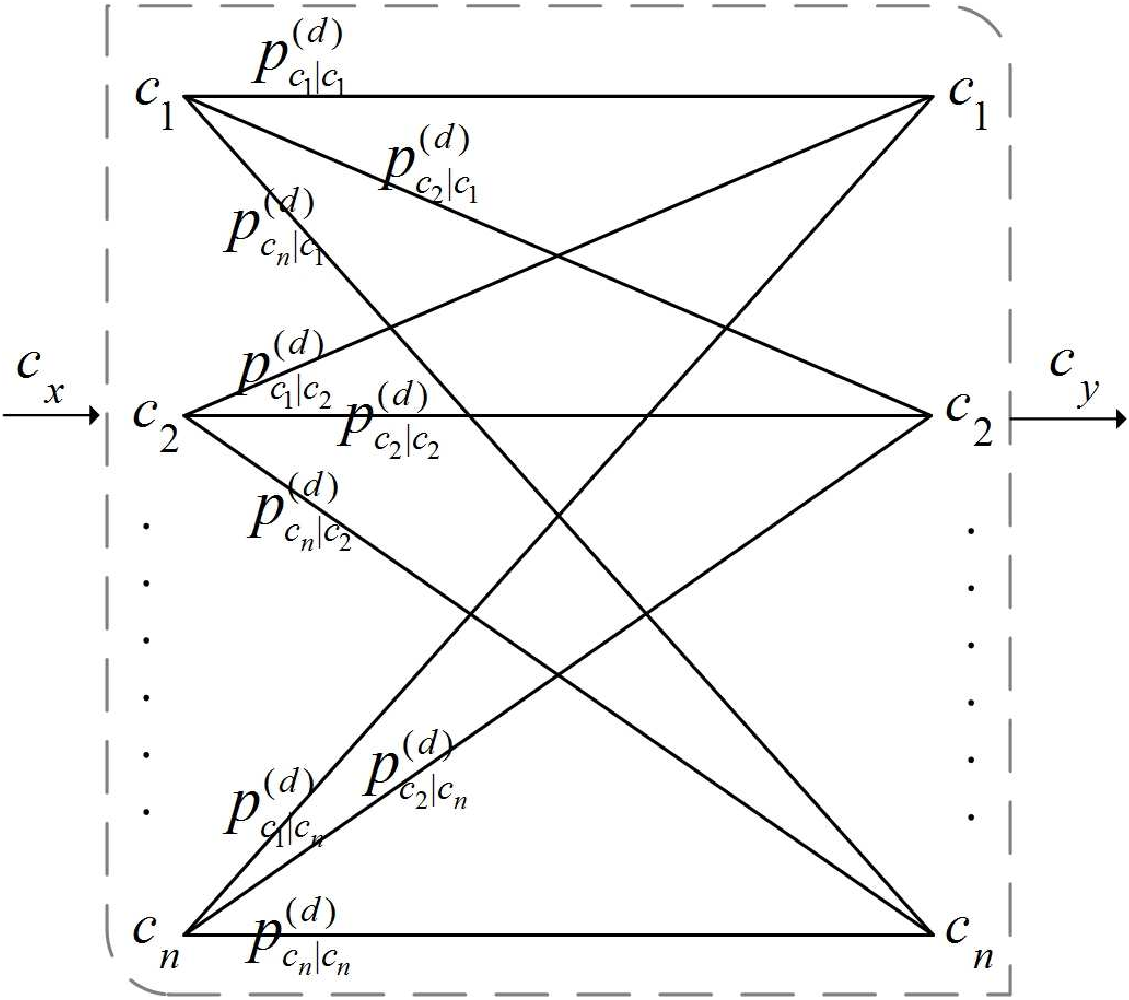
\includegraphics[width=0.75\columnwidth]{d_channel}
    \vspace{0.5cm}
    \caption{Power quality transition at each device $d$ as a channel.}
    \vspace{2cm}
    \label{fig:d_channel}
\end{figure}

Moreover, in order to simplify our model, we treat the power flow through each node as a channel (shown in Figure~\ref{fig:d_channel}). The input and output of this channel at each node comprises $n$ power quality classes. The probability that a power quality $c_x$ will be ``received" as $c_y$ at the output of the channel at each device $d$ is represented by the symbol $p_{c_y  \mid c_x}^{(d)}$. For each device $d$, we call the $n\times n$ matrix consisting of the probability values  $p_{c_y  \mid c_x}^{(d)}$ the \emph{power quality transition function}, or simply \emph{transition function}. For a device (subnet) having multiple inputs/outputs, a power quality transition function is associated with each input/output pair. We represent the power quality transition function $f(d)$ of a device $d$ as a matrix as

\begin{equation}
f(d) = \left[\begin{array}{cccc} p_{c_1 \mid c_1}^{(d)} & p_{c_2 \mid c_1}^{(d)} & \cdots & p_{c_n \mid c_1}^{(d)}\\
p_{c_1 \mid c_2}^{(d)} & p_{c_2 \mid c_2}^{(d)} & \cdots & p_{c_n \mid c_2}^{(d)}\\
\vdots & \vdots& \ddots & \vdots\\
p_{c_1 \mid c_n}^{(d)} & p_{c_2 \mid c_n}^{(d)} & \cdots & p_{c_n \mid c_n}^{(d)}
\end{array}\right],
\label{eqn:pqf}
\end{equation}

\noindent
where $p_{c_y \mid c_x}^{(d)}$ is the probability that the input quality $c_x$ is received as $c_y$ at the output of device $d$. Note that every row in the above matrix should sum to $1$. 

The above model significantly simplifies the network complexity of the power grid. Using this analytical model, in the next few chapters, we propose various algorithms for power quality monitoring and demonstrate that this model significantly simplifies our solutions. A short summary of the proposing algorithms as applications of our analytical model is given in the next section.

\section{Applications}
We build various applications on top of the analytical framework we proposed in this Chapter. The applications are as follows.

\subsection{Power Quality Estimation}
Figure~\ref{fig:gridNetwork} shows a view of a power grid where there are different types of electrical devices connected to each other via power links. The smart meters are also installed on selected links. Moreover, every type of device has a power quality function which may be unknown. We want to estimate all the power quality functions based on the power quality values available on selected links where smart meters are installed.

In order to estimate the reliability of every device in the network, we need to estimate the power quality function $f(d_j)$ for each device $d_j$ based on the quality function $f(s)$ of the subnet. It is clear that

\begin{landscape}
\begin{figure*}[!p]
    \centering
    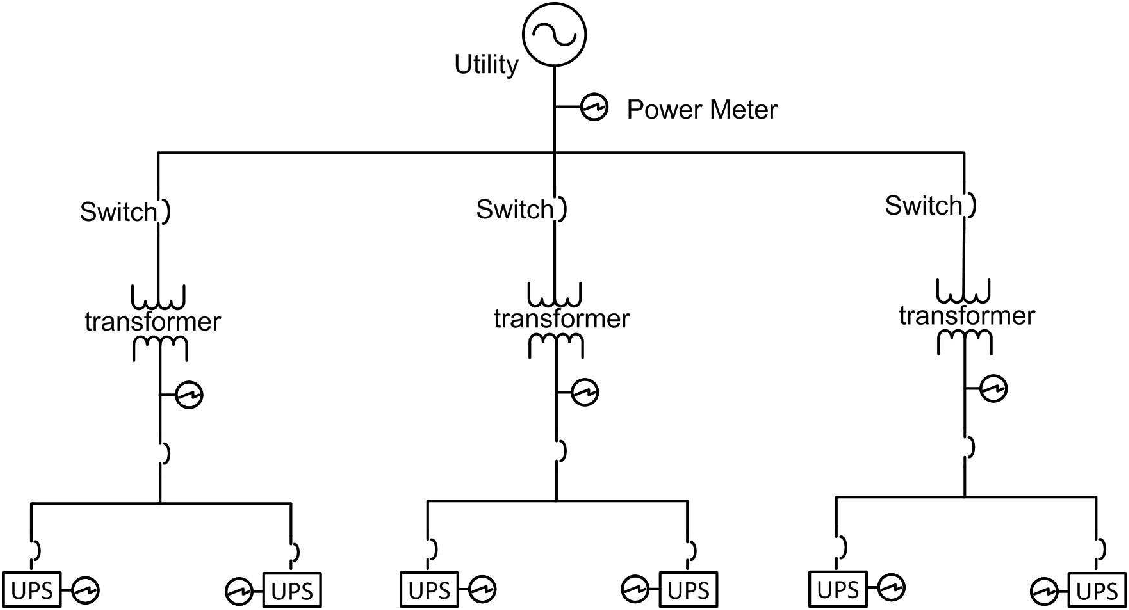
\includegraphics[width=1.2\textwidth]{powerNetwork}
    \vspace{0.5cm}    
    \caption{A simple view of power microgrid}
    \vspace{2cm}
    \label{fig:gridNetwork}
\end{figure*}
\end{landscape}

\begin{equation}
\label{eqn:prod}
f(s) = \prod_{j} f(d_j),
\end{equation}

Our objective is to estimate $p_{c_y \mid c_x}^{(d_j)}$ (probability that power quality $c_x$ will be mapped to power quality $c_y$ at each device $d_j$). In order to solve the above research problem, we model the power network as data network which give us the opportunity to use the already proposed data estimation techniques to solve Eq.~(\ref{eqn:prod}).

\subsection{Intelligent Meter Placement}
For the meter placement problem, we propose an iterative approach for identifying network segments suitable for power meter placement. During each iteration of the algorithm we identify in a greedy manner the network segment that suffers from the most unpredictable power quality given the meters deployed so far. We then deploy the next power meter at that location. Our proposed meter placement algorithms take advantage of our network model to calculate the uncertainty of the power quality values on various network segments.

Similarly, we use the same network model to solve the problem of getting the optimized number of meters required to achieve certain level of reliability. We formulate this problem as an optimization problem where the objective is to reduce the number of meters while maintaining an acceptable level of reliability. In order to calculate the reliability (the uncertainty of power quality) on power links, we use this network model which simplify the representation of the power network as a data network.


\subsection{Detecting a Malfunction Device}
Our third contribution is detecting a malfunction device in the power grid. Since the model we propose to detect a malfunction device uses our meter placement algorithms, the same concept of simplifying the power grid as a data network need to be used here as well. The proposed model is using the exact PQ values from the metered locations and inferred values from the unmetered locations in the network. A device is considered malfunction when it consistently behaving abnormal by generating significantly different PQ values than the expected ones. The acceptable behavior is derived with the help of CBEMA curve.